% Template for ICASSP-2016 paper; to be used with:
%          spconf.sty  - ICASSP/ICIP LaTeX style file, and
%          IEEEbib.bst - IEEE bibliography style file.
% --------------------------------------------------------------------------
% \documentclass{article}
% \usepackage[utf8]{inputenc}
%
% \usepackage{spconf,amsmath,graphicx}
% \usepackage{amstext}
% \usepackage{amssymb}
% \usepackage{float}
% \usepackage{framed}
% \usepackage{booktabs}
% \usepackage{cite}
% \usepackage{enumitem}% http://ctan.org/pkg/enumitem


% \usepackage[unicode=true,
%  bookmarks=true,bookmarksnumbered=false,bookmarksopen=false,
%  breaklinks=false,backref=false,colorlinks=false]
%  {hyperref}
%

% lyx specific stuff

In this paper we present a novel source separation method aiming to overcome the difficulty of modelling non-stationary signals. The method can be applied to mixtures of musical instruments with frequency and/or amplitude modulation, e.g.\ typically caused by vibrato. It is based on a signal representation that divides the complex spectrogram into a grid of patches of arbitrary size. These complex patches are then processed by a two-dimensional discrete Fourier transform, forming a tensor representation which reveals spectral and temporal modulation textures. Our representation can be seen as an alternative to modulation transforms computed on magnitude spectrograms. An adapted factorization model allows to decompose different time-varying harmonic sources based on their particular common modulation profile: hence the name \emph{Common Fate Model}. The method is evaluated on musical instrument mixtures playing the same fundamental frequency (unison), showing improvement over other state-of-the-art methods.

\section{Common Fate Model}

In this section we present a source separation method aiming to overcome the difficulty of modelling non-stationary signals. The method can be applied to mixtures of musical instruments with frequency and/or amplitude modulation, e.g.\ typically caused by vibrato. It is based on a signal representation that divides the complex spectrogram into a grid of patches of arbitrary size. These complex patches are then processed by a two-dimensional discrete Fourier transform, forming a tensor representation which reveals spectral and temporal modulation textures. Our representation can be seen as an alternative to modulation transforms computed on magnitude spectrograms. An adapted factorization model allows to decompose different time-varying harmonic sources based on their particular common modulation profile: hence the name \emph{Common Fate Model}. The method is evaluated on musical instrument mixtures playing the same fundamental frequency (unison), showing improvement over other state-of-the-art methods.

\label{sec:model}

\subsection{The Common Fate Transform}

\label{sub:CFT}

Let $\tilde{x}$ denote a single channel audio signal.
Its Short-Term Fourier Transform (STFT) is computed by splitting it
into overlapping frames, and then taking the discrete Fourier transform (DFT)
of each one\footnote{Since the waveform~$\tilde{x}$ is real, the Fourier transform of
each frame is Hermitian. In the following, we assume that the redundant
information has been discarded to yield the STFT.}. The resulting information is gathered into an $N_{\omega}\times N_{\tau}$
matrix written~$X$, where~$N_{\omega}$ is the number of frequency
bands and $N_{\tau}$ the total number of frames.
%
In this study, we will consider the properties of another object,
built from $X$, which we call the Common Fate Transform (CFT). It
is constructed as illustrated in Figure~\ref{fig:CFT}.
We split the STFT~$X$ into overlapping rectangular $N_{a}\times N_{b}$
patches, regularly spaced over both time and frequency. Then, the
2D-DFT of each patch is computed\footnote{Note that since each patch is complex, its 2D-DFT is not Hermitian,
thus all its entries are kept.}. This yields an $N_{a}\times N_{b}\times N_{f}\times N_{t}$ tensor we write~$x$,
where~$N_{f}$ and~$N_{t}$ are the vertical and horizontal
positions for the patches, respectively.

As can be seen, the CFT is basically a further short-term 2D-DFT taken over
the standard STFT~$X$. One of the main differences compared to modulation spectrograms
is that the CFT is computed using the complex STFT~$X$, and not a magnitude representation such as $\left|X\right|$. As we will
show, this simple difference has many interesting consequences, notably
that the CFT is invertible: the original waveform~$\tilde{x}$ can
be exactly recovered by cascading two classical overlap-add procedures. Another difference
is that the patches span several frequency bins, \emph{i.e.} we may have~$N_{a}>1$.
This contrasts with the conventional modulation spectrogram, that
is usually defined using one frequency band only.

\begin{figure}[t]
\centering
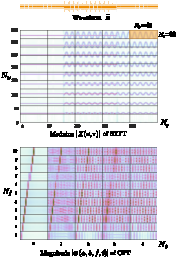
\includegraphics[width=0.9\columnwidth]{Chapters/commonfate/figures/CFT}

\caption{Common Fate Transform. For convenience, the splitting of the STFT
into patches has been depicted without overlap, but overlapping patches
are used in practice\label{fig:CFT}.}
\end{figure}

\subsection{A Probabilistic Model for the CFT}

\label{sub:separation}

When processing an audio signal~$\tilde{x}$ for source separation,
it is very common to assume that all time-frequency (TF) bins
of its STFT are independent~\cite{fevotte09,duong10,ozerov12,liutkus11t}.
This is often the consequence of two different assumptions.
The first one is to consider that all frames are independent, thus
leading to the independence of all entries of the STFT that do not belong to the
same column. The second one is related to the notion of stationarity:
roughly speaking, the Fourier transform is known to decompose stationary
signals into independent components, whether these signals be Gaussian
(see, e.g.~\cite{liutkus11t}) or, more generally, harmonisable $\alpha$-stable~\cite{liutkus15}.
As a consequence, when the signals are assumed to be \emph{locally stationary},
it is theoretically sound to assume that all the entries of
their STFT are independent.

Still, both assumptions can only be considered as approximations.
First, adjacent frames are obviously not independent, notably because
of the overlap between them. Second, the stationarity assumption is
only approximate in practice, especially when impulsive elements are
found in the audio, leading to strong dependencies among the different
frequency bins. Let $\{ X_{ft}\} _{f,t}$
denote all the $N_{a}\times N_{b}$ patches taken on the STFT to compute
the CFT, as depicted in Figure~\ref{fig:CFT}. The probabilistic
model we choose is the combination of \emph{four} different assumptions
made on the distribution of these patches.

\begin{enumerate}[leftmargin=0cm,itemindent=.5cm,labelsep=0cm,align=left]
\item All patches are independent. Just as the classical locally stationary
model~\cite{liutkus11t} assumes independence of overlapping frames,
we assume here independence of overlapping patches. Due to the
overlap between them, this assumption is an approximation,
and one may wonder what the advantage is of dropping independent frames
for independent patches. The answer lies in the fact that the latter
permits us to model phase dependencies between neighbouring STFT entries,
and also to model much longer-term dependencies, as required for instance
by deterministic damped or frequency-modulated sinusoidal signals.\label{enu:assumption_independent_patches}
\item Each patch is \emph{stationary}: its distribution
is assumed invariant under translations in the TF plane. This is where we do not assume independence, but on the contrary expect dependencies among neighbouring STFT entries. Our approach assumes this happens in a way that only depends on the relative positions in
the TF plane. It can easily be shown that mixtures of
damped sinusoids have this property. Assuming stationarity not only over time but over both time and frequency
also permits us to naturally account for mixtures of frequency-modulated
sounds. In short, we assume that throughout each patch, we observe
one coherent STFT ``texture''. The difference with the HR-NMF model is that we have independent and identically
distributed (i.i.d.) innovations for one given patch, whereas HR-NMF model has more variability and permits heteroscedastic innovations. However, taking overlapping patches somehow compensates for
this limitation.\label{enu:assumption_stationary}
\item The joint distribution of all entries of each patch is $\alpha$-stable~\cite{samoradnitsky1994stable}.
$\alpha$-stable distributions are the only ones that are stable under additions, \emph{i.e.} such that
sums of $\alpha$-stable random variables (r.v.) remain $\alpha$-stable.
They notably comprise the Gaussian and Cauchy distributions as special
cases when $\alpha=2$ and $\alpha=1$, respectively.\label{enu:assumption_alpha_stable}
\item Each patch is harmonisable, \emph{i.e.} is the inverse Fourier
transform of a complex random measure with independent increments.
In other words, all entries of the Fourier transform of each patch
are assumed to be asymptotically independent, as the size of the patch
gets larger. This rather technical condition, often tacitly made in
signal processing studies, permits efficient processing in the frequency
domain.\label{enu:assumption_harmonisable}
\end{enumerate}

Under those four assumptions, all entries of the CFT~$x$ are independent
(assumptions~\ref{enu:assumption_independent_patches} and~\ref{enu:assumption_stationary}),
and each one is distributed with respect to a complex isotropic $\text{\ensuremath{\alpha}}$-stable
distribution, noted $S\alpha S_{c}$ (assumptions~\ref{enu:assumption_alpha_stable}
and~\ref{enu:assumption_harmonisable}\footnote{This result is the direct generalization
of~\cite[th. 6.5.1]{samoradnitsky1994stable} to multi-dimensional stationary processes.}):
\begin{equation}
x\left(a,b,f,t\right)\sim S\alpha S_{c}\left(P^{\alpha}\left(a,b,f,t\right)\right),\label{eq:SaS_model}
\end{equation}
where $P^{\alpha}$ is a nonnegative $N_{a}\times N_{b}\times N_{f}\times N_{t}$
tensor that we call the \emph{modulation density}. When $\alpha=2$,~\eqref{eq:SaS_model}
corresponds to the classical isotropic complex Gaussian distribution
and the entries of $P^{\alpha}$ are homogeneous to variances. In
the general case, it can basically be understood as the energy found at $\left(a,b\right)$ for patch
$\left(f,t\right)$, just like more classical (fractional) power spectral
densities describe the spectro-temporal energy content of the STFT
of a locally stationary signal.

% \subsection{Another interpretation of the CFT}
%
% \label{sub:interpretation}

An alternative interpretation of the CFT can be obtained by regarding the 2D-DFT
as two subsequent 1D-DFTs. If the transform in frequency direction (DFT-F) is
applied first, it is equivalent to a partial inverse DFT plus time reversal. If
the time reversal would be undone and an overlap-add would be applied, the
output would correspond to a subband representation with a frequency resolution
of $N_\omega / N_a$. Each of the $N_a$ final transformations (DFT-T) in one
patch takes output values from $N_b$ DFT-Ts with equal indices. This corresponds
to a splitting into poly-phase components with downsampling factor $N_a$ of the
time signal obtained by placing the output frames from the DFT-Ts in a row.
Thus, the outputs of the DFT-Fs have a very high frequency resolution of
$N_\omega N_b$ but contain aliasing components from the downsampling.

This interpretation of the CFT gives some indications for its benefits in the
separation of modulated sources. Due to the poly-phase representation it has a
relatively high temporal resolution. The periodicities in the spectra caused
by downsampling make the CFT relatively independent of frequency shifts, so
that, for example, the output patch of a single sinusoidal sweep is mainly
influenced by the sweep rate.

\subsection{Factorization Model for Signal Separation}

Now, let us assume that the observed waveform is actually the sum
of~$J$ underlying sources~$\{ \tilde{s}_{j}\} _{j=1,\dots,J}$.
Due to the linearity of the CFT, this can be
expressed in the CFT domain as:
$$
\forall\left(a,b,f,t\right),x\left(a,b,f,t\right)=\sum\nolimits_{j}s_{j}\left(a,b,f,t\right).
$$
If we adopt the $\alpha$-stable model presented above for each source
and use the stability property, we have:
$$
x\left(a,b,f,t\right)\sim S\alpha S_{c}\left(\sum\nolimits_{j}P_{j}^{\alpha}\left(a,b,f,t\right)\right),
$$
where $P_{j}^{\alpha}$ is the modulation density for source~$j$.
If these objects are known, it can be shown that each source can be
estimated in a maximum a posteriori sense from the mixture as:
\begin{equation}
\mathbb{E}\left[s_{j}\left(a,b,f,t\right)\mid \{ P_{j}^{\alpha}\} _{j},x\right]=\tfrac{P_{j}^{\alpha}\left(a,b,f,t\right)}{\sum_{j'}P_{j'}^{\alpha}\left(a,b,f,t\right)} \, x\left(a,b,f,t\right)\label{eq:alpha_wiener}
\end{equation}
which we call the fractional $\alpha$-Wiener filter in~\cite{liutkus15}.
The resulting waveforms are readily obtained by inverting the CFT.\@
As can be seen, we now need to estimate the modulation
densities~$\{ P_{j}^{\alpha}\} _{j}$ based on the observation
of the mixture CFT~$x$, similarly to the estimation of
 the sources' (fractional) Power Spectral Densities ($\alpha$-PSD)
in source separation studies.


% \subsection{Factorization Model and Parameter Estimation}

\label{sub:NTF}

In order to estimate the sources' modulation densities, we first impose
a factorization model over them, so as to reduce the number of parameters
to be estimated. In this study, we set:
\begin{equation}
P_{j}^{\alpha}\left(a,b,f,t\right)=A_{j}\left(a,b,f\right)H_{j}\left(t\right),\label{eq:NTF_model}
\end{equation}
where $A_{j}$ and $H_{j}$ are $N_{a}\times N_{b}\times N_{f}$ and~$N_{t}\times1$
nonnegative tensors, respectively. We call this a \emph{Common Fate
Model}. Intuitively, $A_{j}$ is a modulation density template that
is different for each frequency band~$f$, and that captures the
long term modulation profile of source~$j$ around that frequency.
Then, $H_{j}$ is an activation vector that indicates the strength
of source~$j$ on the patches located at temporal position~$t$.
Learning those parameters can be achieved using the conventional Nonnegative
Matrix Factorization methodology (NMF, see e.g.~\cite{cichoki09,ozerov12,smaragdis14}
for an overview and~\cite{liutkus15b} for the fitting of $S\alpha S_{c}$
parameters), except that it is applied to the CFT instead of the STFT,
and that the particular factorization to be used is~\eqref{eq:NTF_model}.

Due to space constraints, we cannot detail the derivations of the
fitting strategy. In essence, it amounts to estimating the parameters~$\{ A_{j},H_{j}\} $
so that the modulus of the CFT, raised to the power $\alpha$, is
as close as possible to~$\sum_{j}P_{j}^{\alpha}$, with some particular
cost function as a data-fit criterion, called a $\beta$-divergence
and which includes Euclidean, Kullback-Leibler and Itakura-Saito as
special cases~\cite{fitzgerald08a}. As usual in such nonnegative models,
each parameter is updated in turn, while the others are kept fixed.
We provide the multiplicative updates in Algorithm~\ref{alg:Fitting-NTF}.
After a few iterations, the parameters can be used in~\eqref{eq:alpha_wiener} to separate
the sources.

\begin{algorithm}
With $v^{\alpha}=\left|x\right|^{\alpha}$ and always using the latest
parameters available for computing
 $\hat{P}^{\alpha}\left(a,b,f,t\right)=\sum\limits_{j=1}^{J}A_{j}\left(a,b,f\right)H_{j}\left(t\right)$,
iterate:
\[
A_{j}\left(a,b,f\right)\leftarrow A_{j}\left(a,b,f\right)\tfrac{\sum_{t}v^{\alpha}\left(a,b,f,t\right)\hat{P}^{\alpha}\left(a,b,f,t\right)^{\cdot\left(\beta-2\right)}H_{j}\left(t\right)}{\sum_{t}\hat{P}^{\alpha}\left(a,b,f,t\right)^{\cdot\left(\beta-1\right)}H_{j}\left(t\right)}
\]
\[
H_{j}\left(t\right)\leftarrow H_{j}\left(t\right)\tfrac{\sum_{a,b,f}v^{\alpha}\left(a,b,f,t\right)\hat{P}^{\alpha}\left(a,b,f,t\right)^{\cdot\left(\beta-2\right)}A_{j}\left(a,b,f\right)}{\sum_{a,b,f}\hat{P}^{\alpha}\left(a,b,f,t\right)^{\cdot\left(\beta-1\right)}A_{j}\left(a,b,f\right)}.
\]


\caption{Fitting NMF parameters of the nonnegative CFM~\eqref{eq:NTF_model}.\label{alg:Fitting-NTF}}
\end{algorithm}

%!TEX root = ../icassp2016.tex
\section{Experiments}
\label{sec:experiment}

\begin{table*}[ht!]
  \centering
\begin{tabular}{ llll }
    \toprule
    Method & Description & Signal Representation & Factorization Model \\
    \midrule
    CFM & Common Fate Model & STFT $\rightarrow$ Grid Slicing $\rightarrow$ 2D-DFT & $V(a,b,f,t) = P(a,b,f)\times H(t)$ \\
    NMF &\cite{virtanen07} w/o add.\ constraints & STFT & $V(f,t) = W(f)\times H(t)$ \\
    HR-NMF & High Resolution NMF model~\cite{magron15a} & Output of any filterbank (STFT, MDCT, \ldots)  & Subband AR filtering of NMF excitation \\
    MOD &\cite{barker13} using DFT filterbank& STFT $\rightarrow$ $|\ldots|$ $\rightarrow$ STFT along each bin & $V(f,m,t) = W(f)\times A(m)\times H(t)$ \\
    CFMM & Common Fate Magnitude Model & STFT $\rightarrow$ $|\ldots|$ $\rightarrow$ Grid Slicing $\rightarrow$ 2D-DFT & $V(a,b,f,t) = P(a,b,f)\cdot H(t)$ \\
    CFMMOD & CFMM with $a=1$ & STFT $\rightarrow$ $|\ldots|$ $\rightarrow$ Grid Slicing $\rightarrow$ 2D-DFT & $V(a,b,f,t) = P(a,b,f)\cdot H(t)$ \\
    \bottomrule
\end{tabular}
\caption{Overview of the evaluated algorithms}
\label{tab:methods}
\end{table*}

In this section, we present separation experiments utilizing CFM and we compare it with other methods.

% \subsection{Synthetic Example}
% \label{sub:Synthentic_Examples}

To illustrate the CFT representation we processed a mixture consisting of two sinusoidal sources. One source is a pure sine wave of fundamental frequency 440~Hz whereas the other is frequency modulated by a sinusoid of 6.3~Hz. In the first step an STFT with a DFT-length of 1024 samples and a hop-size of 256 samples was processed at a sample rate of 22.05~kHz. Patches of size $(N_a, N_b) = (32, 48)$ (not respecting overlaps) were then taken from the STFT output. Figure~\ref{fig:CFT} in Section~\ref{sub:CFT} then shows the Common Fate Transform for the mixture as described in Section~\ref{sec:model}. One can see that the CFT representation shows distinct patterns across time, suggesting that the factorization is able to separate the sources.

\begin{figure}[b]
\centering
		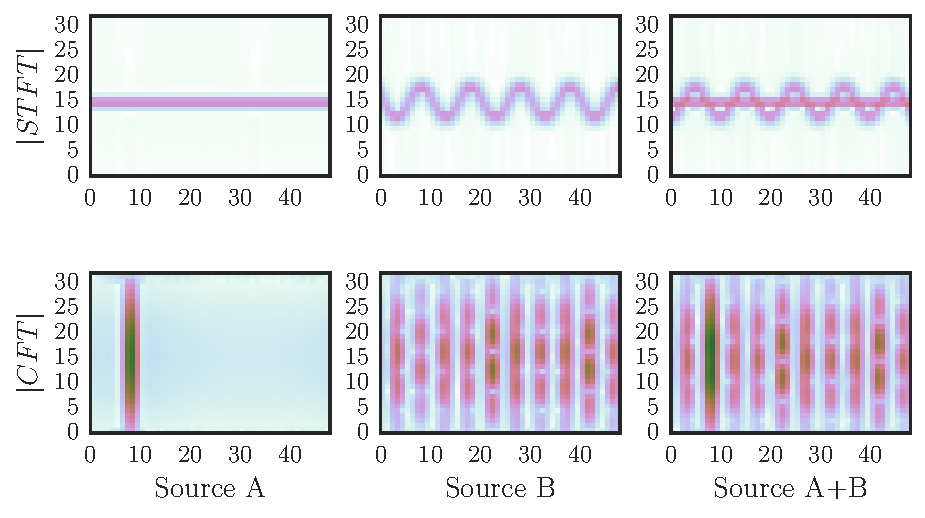
\includegraphics[width=0.95\columnwidth]{Chapters/commonfate/figures/gridplot.pdf}
\caption{Examples of patches of size $(N_a, N_b) = (32, 48)$. The upper row shows magnitude values from the STFT output, the lower row the corresponding Common Fate Transform (CFT).}
\label{fig:gridplot}
\end{figure}

% \subsection{Objective Evaluation on Unison Instrument Mixtures}

For an evaluation of the method, we selected five musical instruments' samples, all featuring vibrato: violin, cello, tenor sax, English horn, and flute. It is important to note that vibrato techniques differ between instruments: whereas the English horn and the flute only produce a very subtle modulation, the violin and tenor sax have powerful frequency modulations with a higher modulation frequency as well as a higher modulation index. The signals have each been generated by rendering C4 (261.63~Hz) notes in a state-of-the-art software sampler\footnote{\textsc{Vienna Symphonic Library} (\url{https://vsl.co.at})}. All samples last about three seconds. We then generated a combination of ten mixtures of two instruments each, each one generated with a simple SourceA --- SourceB --- (SourceA + SourceB) scheme. Data were encoded in 44.1 kHz / 16 bit.
For evaluation, we compared separation performance of six different methods, summarized in Table~\ref{tab:methods}:
\begin{description}[style=unboxed,leftmargin=0cm]
\item[CFM] For the CFM model, we took an STFT with frames of 1024 samples and a hop-size of 512 samples. The resulting complex spectrogram was then split into a grid of patches of size $(N_a, N_b) = (4, 64)$, each having a half-window overlap in both dimensions. For all experiments $\alpha$ and $\beta$ were set to 1.
\item[MOD] We implemented a modified version of~\cite{barker13} where for the sake of comparability, we used a STFT instead of a gammatone filterbank. A DFT length of 1024 and a hop-size of 512 samples were chosen. After taking the magnitude value, a second STFT of size 32 and hop-size 16 samples was computed for each frequency.
\item[CFMMOD] We selected patch sizes of $(N_a, N_b) = (1, 64)$ and modified the representation so that the magnitude spectrogram was used before computing the 2D-DFT.\@ This permits to compare the advantage of our proposed factorization model~(\ref{eq:NTF_model}) over MOD, when using the same kind of energy-modulation representation in both cases.
\item[CFMM] For comparing the influence of computing modulations over complex STFT or magnitude spectrograms, we tried our factorization model when the magnitude of the STFT is taken before 2D-DFT, with patches of the same size as for the CFM method.
\item[NMF] We took a standard NMF based method~\cite{virtanen07}. We highlight that taking a spectrogram with frames of length 1024 would not make a fair comparison, because the CFM model actually results in a larger frequency resolution. Therefore a comparable NMF is based on an STFT of DFT-length 32768.
\item[HR-NMF] See description in~\cite{magron15a}.
\end{description}
All factorizations ran for 100 iterations and were repeated five times. We chose $j=(2\ldots6)$ components for each factorization. For $j > 2$ we used oracle clustering to show the upper limit of SDR which can be achieved.

We ran the performance evaluation by using BSSeval~\cite{Vincentbsseval06}. The results of Signal to Distortion
Ratio (SDR), Signal to Interference Ratio (SIR), and Signal to Artifacts Ration (SAR) are depicted in Figure~\ref{fig:boxplot_overall}. Results indicate that the CFM model performs well in all measures. However, in terms of SIR the results of HR-NMF are better than CFM method. The results for CFMMOD indicate the positive influence of the CFM factorization compared to~\cite{barker13}.
The results of CFMM indicate that the complex CFT lead to better results. NMF did perform surprisingly well, which may only hold for our test set, where each source is active for a long period. This results in a cyclic stationary vibrato, revealing spectral side lobes at such a high resolution. With more than one component per source, the results of CFM do improve, but it can be seen that more than two components ($j=4$) will not increase the SDR values. The separation results and a full Python implementation of the CFM algorithm can be found on the companion website for this paper\footnote{\url{www.loria.fr/~aliutkus/cfm/}}.

To understand the influence of the underlying matrix or tensor representation we additionally computed a normalized tensor correlation for each of the methods before before applying the factorization. Therefore for each source we compute the sum of the Hadamard product and normalize the output to the it's energy. The mean results of this correlation are shown in table~\ref{tab:correlation}.

\begin{figure}[ht!]
\centering
		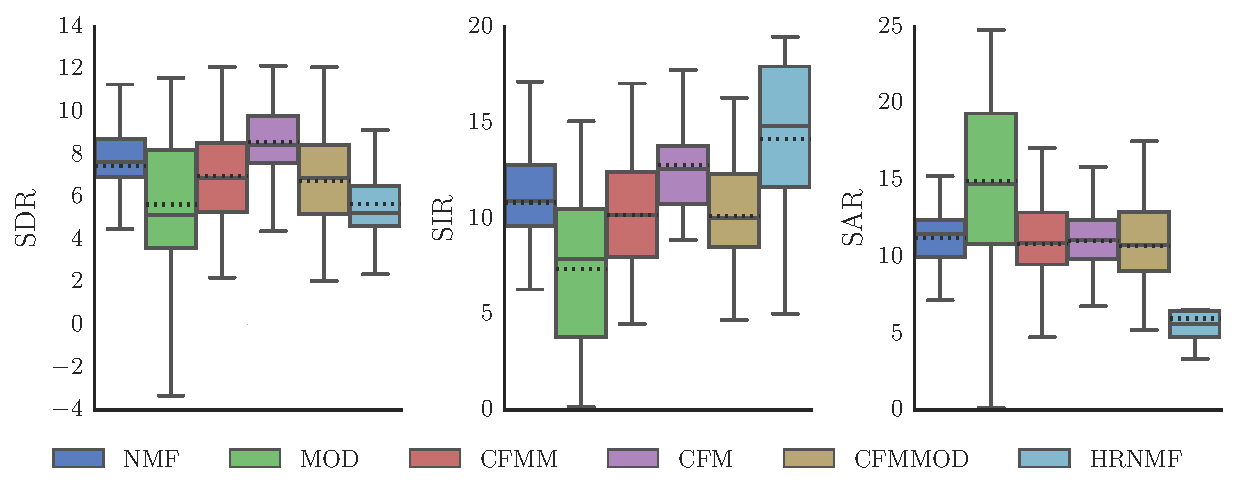
\includegraphics[width=0.90\columnwidth]{Chapters/commonfate/figures/boxplot.pdf}
\caption{Boxplots of BSS-Eval results of the unison dataset. Solid/dotted lines represent medians/means.}
\label{fig:boxplot_overall}
\end{figure}

\begin{figure}[ht!]
\centering
		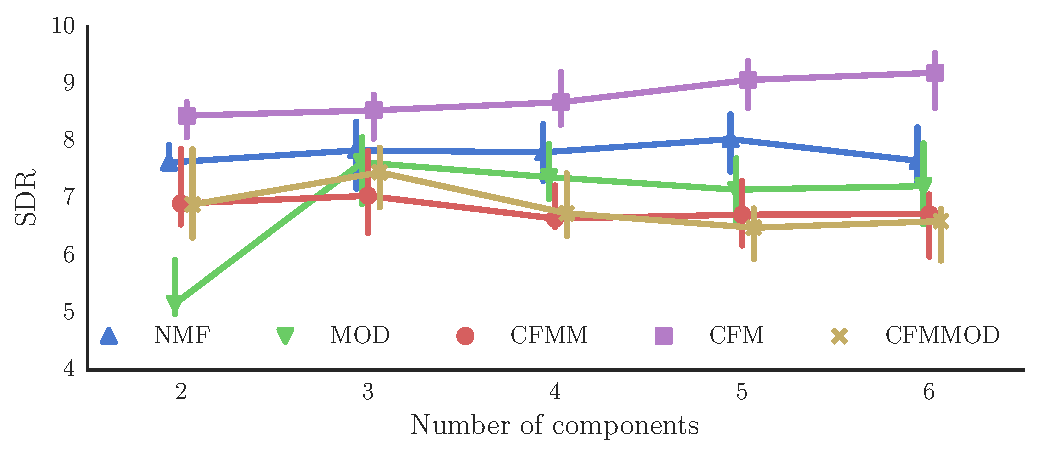
\includegraphics[width=0.90\columnwidth]{Chapters/commonfate/figures/iterations.pdf}
\caption{Boxplots of SDR values of the unison dataset over the number of components $j$. For $j>2$ oracle clustering was applied.}
\label{fig:iterations}
\end{figure}

\section{Conclusion}
\label{sec:conclusion}

In this work we presented a method to exploit common modulation textures for source separation. A transformation based on a complex tensor representation computed from patches of the STFT has been introduced. We then showed how these patches are factorized by the proposed \emph{Common Fate Model}, which is derived from the idea of humans perceiving common modulation over time as one source. Our results on unisonous musical instruments indicate that this method can perform well for this scenario. The CFM model could also be successfully used in other scenarios, such as speech separation.
